\documentclass[12pt,fleqn]{article}\usepackage{../../common}
\begin{document}
Hareketin Katı-Gövde Denklemleri - 3

Bir diferansiyel denklemi entegre edebilmek için Runge-Kutta yaklaşımının
kodlamasını detaylı şekilde anlamak gerekiyor. RK yaklaşımını [3]'te gördük.
Şimdi Runge-Kutta dördüncü derece çözüm yaklaşımını bir örnekte görelim.

Sarkaç Problemi

Bağlantı noktasında sürtünme içerebilecek basit bir şarkaçın hareket denklemleri
[1, sf. 842],

$$
\ddot{\theta} + b\dot{\theta}  c\sin(\theta) = 0, \quad
t \ge 0, \theta(0)=\theta_0, \quad
\dot{\theta} = \dot{\theta}_0
\mlabel{1}
$$

olarak verilebilir. Bu denklemi ODE sistemi ölarak çözmek için yeni değişken
tanımları üzerinden onu iki parçaya ayırıyoruz,

$$
\vec{x} = x = \left[\begin{array}{ccc}
x_1 \\ x_2
\end{array}\right] = 
\left[\begin{array}{c}
\theta \\ \dot{\theta}
\end{array}\right], \quad
f(t,x) = \left[\begin{array}{c}
\dot{\theta} \\ -b \dot{\theta} - c\sin\theta
\end{array}\right]
$$

Bu tanimlarla $\dot{x}$ ifadesi
$
\dot{x} = \left[\begin{array}{c} \dot{\theta} \\ \ddot{\theta} \end{array}\right]
$
haline gelir,  ve $\dot{x} = f(t,x)$ matris denkleminde 

$$
\left[\begin{array}{c} \dot{\theta} \\ \ddot{\theta} \end{array}\right]=
\left[\begin{array}{c} \dot{\theta} \\ -b \dot{\theta} - c\sin\theta \end{array}\right]
$$

alt satıra odaklanırsak, orada (1) denklemine geri gidebileceğimizi görebiliriz.

Sayısal çözüme gelirsek, benzer bir problemin çözümünü [2]'de işlemiştik.  O
derste bir paket çağrısı olan \verb!odeint! kullanılmıştı, bu paketin
entegrasyonu nasıl yaptığından bahsedilmemişti. Şimdi daha detaylandıralım,
\verb!odeint! kodu iç mantığında dördünce derece Runge-Kutta çözümü kullanır,
yani RK4 yaklaşımını.

\begin{minted}[fontsize=\footnotesize]{python}
n = 256; theta0 = 0.1; dtheta0 = 1.0; h = 0.1; c = 1.0

theta_values = np.zeros(n)

for i in range(n):
    K1theta = h * dtheta0
    K1dtheta = -h * c * np.sin(theta0)
    theta1 = theta0 + 0.5 * K1theta
    dtheta1 = dtheta0 + 0.5 * K1dtheta
    K2theta = h * dtheta1
    K2dtheta = -h * c * np.sin(theta1)

    theta1 = theta0 + 0.5 * K2theta
    dtheta1 = dtheta0 + 0.5 * K2dtheta
    K3theta = h * dtheta1
    K3dtheta = -h * c * np.sin(theta1)
    theta1 = theta0 + K3theta
    dtheta1 = dtheta0 + K3dtheta
    K4theta = h * dtheta1
    K4dtheta = -h * c * np.sin(theta1)
    theta1 = theta0 + (K1theta + 2.0 * K2theta + 2.0 * K3theta + K4theta) / 6.0
    dtheta1 = dtheta0 + (K1dtheta + 2.0 * K2dtheta + 2.0 * K3dtheta + K4dtheta) / 6.0
    theta_values[i] = theta1
    theta0 = theta1
    dtheta0 = dtheta1

plt.ylim(-1.20,1.20)
plt.plot(range(n), theta_values)
plt.savefig('phy_005_basics_06_01.jpg')
\end{minted}

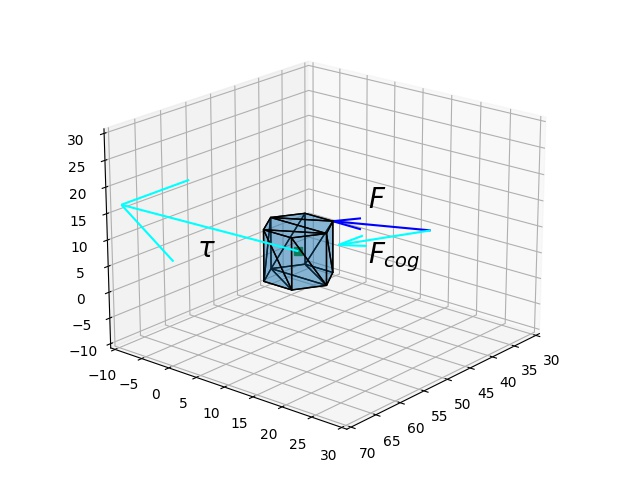
\includegraphics[width=20em]{phy_005_basics_06_01.jpg}












[devam edecek]

Kaynaklar

[1] Eberly, {\em Game Physics 2nd Ed}

[2] Bayramlı, {\em Gayrı-Lineer Dinamik ve Kaos Ders 1}

[3] Bayramlı, {\em Diferansiyel Denklemler Ders 2}

\end{document}
